\documentclass{report}
\usepackage[utf8]{inputenc}
\usepackage{amsmath}
\usepackage{indentfirst}
\usepackage{multirow}
\usepackage{graphicx}
\usepackage{float}
\usepackage[brazil]{babel}
\usepackage{enumitem}

\author{Renan Turrissi}
\date{\today}
\title{Uma Nova Maneira de se Enforcar EM \LaTeX !!!}

\newcommand{\vetor}[1]{\textbf{#1}}

\begin{document}

\maketitle

\chapter{Introdução}\label{chap:intro}
Neste trabalho mostraremos como se enforcar eficientemente.

AAA
% aqui eu tenho que melhorar esse troço

\chapter{Motivação}\label{chap:motiv}
As pessoas se enforcam muito mal hoje em dia.\\
Referencia à introdução: \ref{chap:intro}...\\
Uma fórmula maluca: $ V =RI $   

\hfill

Outra fórmula maluca: $ I = \frac{V}{R} $

$$ 0 = 1+e^{j\pi}  $$


O pé direito é maluco
\footnote[2]{nota de rodapé do pé direito}\\


IDFT: 
\begin{equation} \label{eq:IDFT}
 x_n = \frac{1}{N}\sum_{k=0}^{N-1} X_k \cdot e^{i2\pi kn/N} 
\end{equation}

referência à equação acima: \ref{eq:IDFT}.

Equação dos nerds:
\begin{align}
\label{eq:maxwell1}
\nabla \cdot E & = \frac{\rho}{\epsilon_0} \\
\nabla  & = 0 \\
\nabla \times E & = -\frac{\partial \vetor{B}}{\partial t}
\end{align}

referencia denovo: \ref{eq:maxwell1}. \\

A tabela show:

\begin{table}[!htb] \label{tab:TabelaShow}
	\centering
	\begin{tabular}{c|c}
	\hline
	
	Faixa etária & Altura (cm) \\ \hline
	18 anos & 172,6 \\
	19 anos & 172,0 \\
	20 a 24 anos & 173,0 \\
	25 a 29 anos & 173,0 \\
	30 a 35 anos & 171,6 \\
	\hline
	\end{tabular}
	\caption{Legenda da Tabela}
\end{table}

A figura show:

\begin{figure}[H]
	\centering
	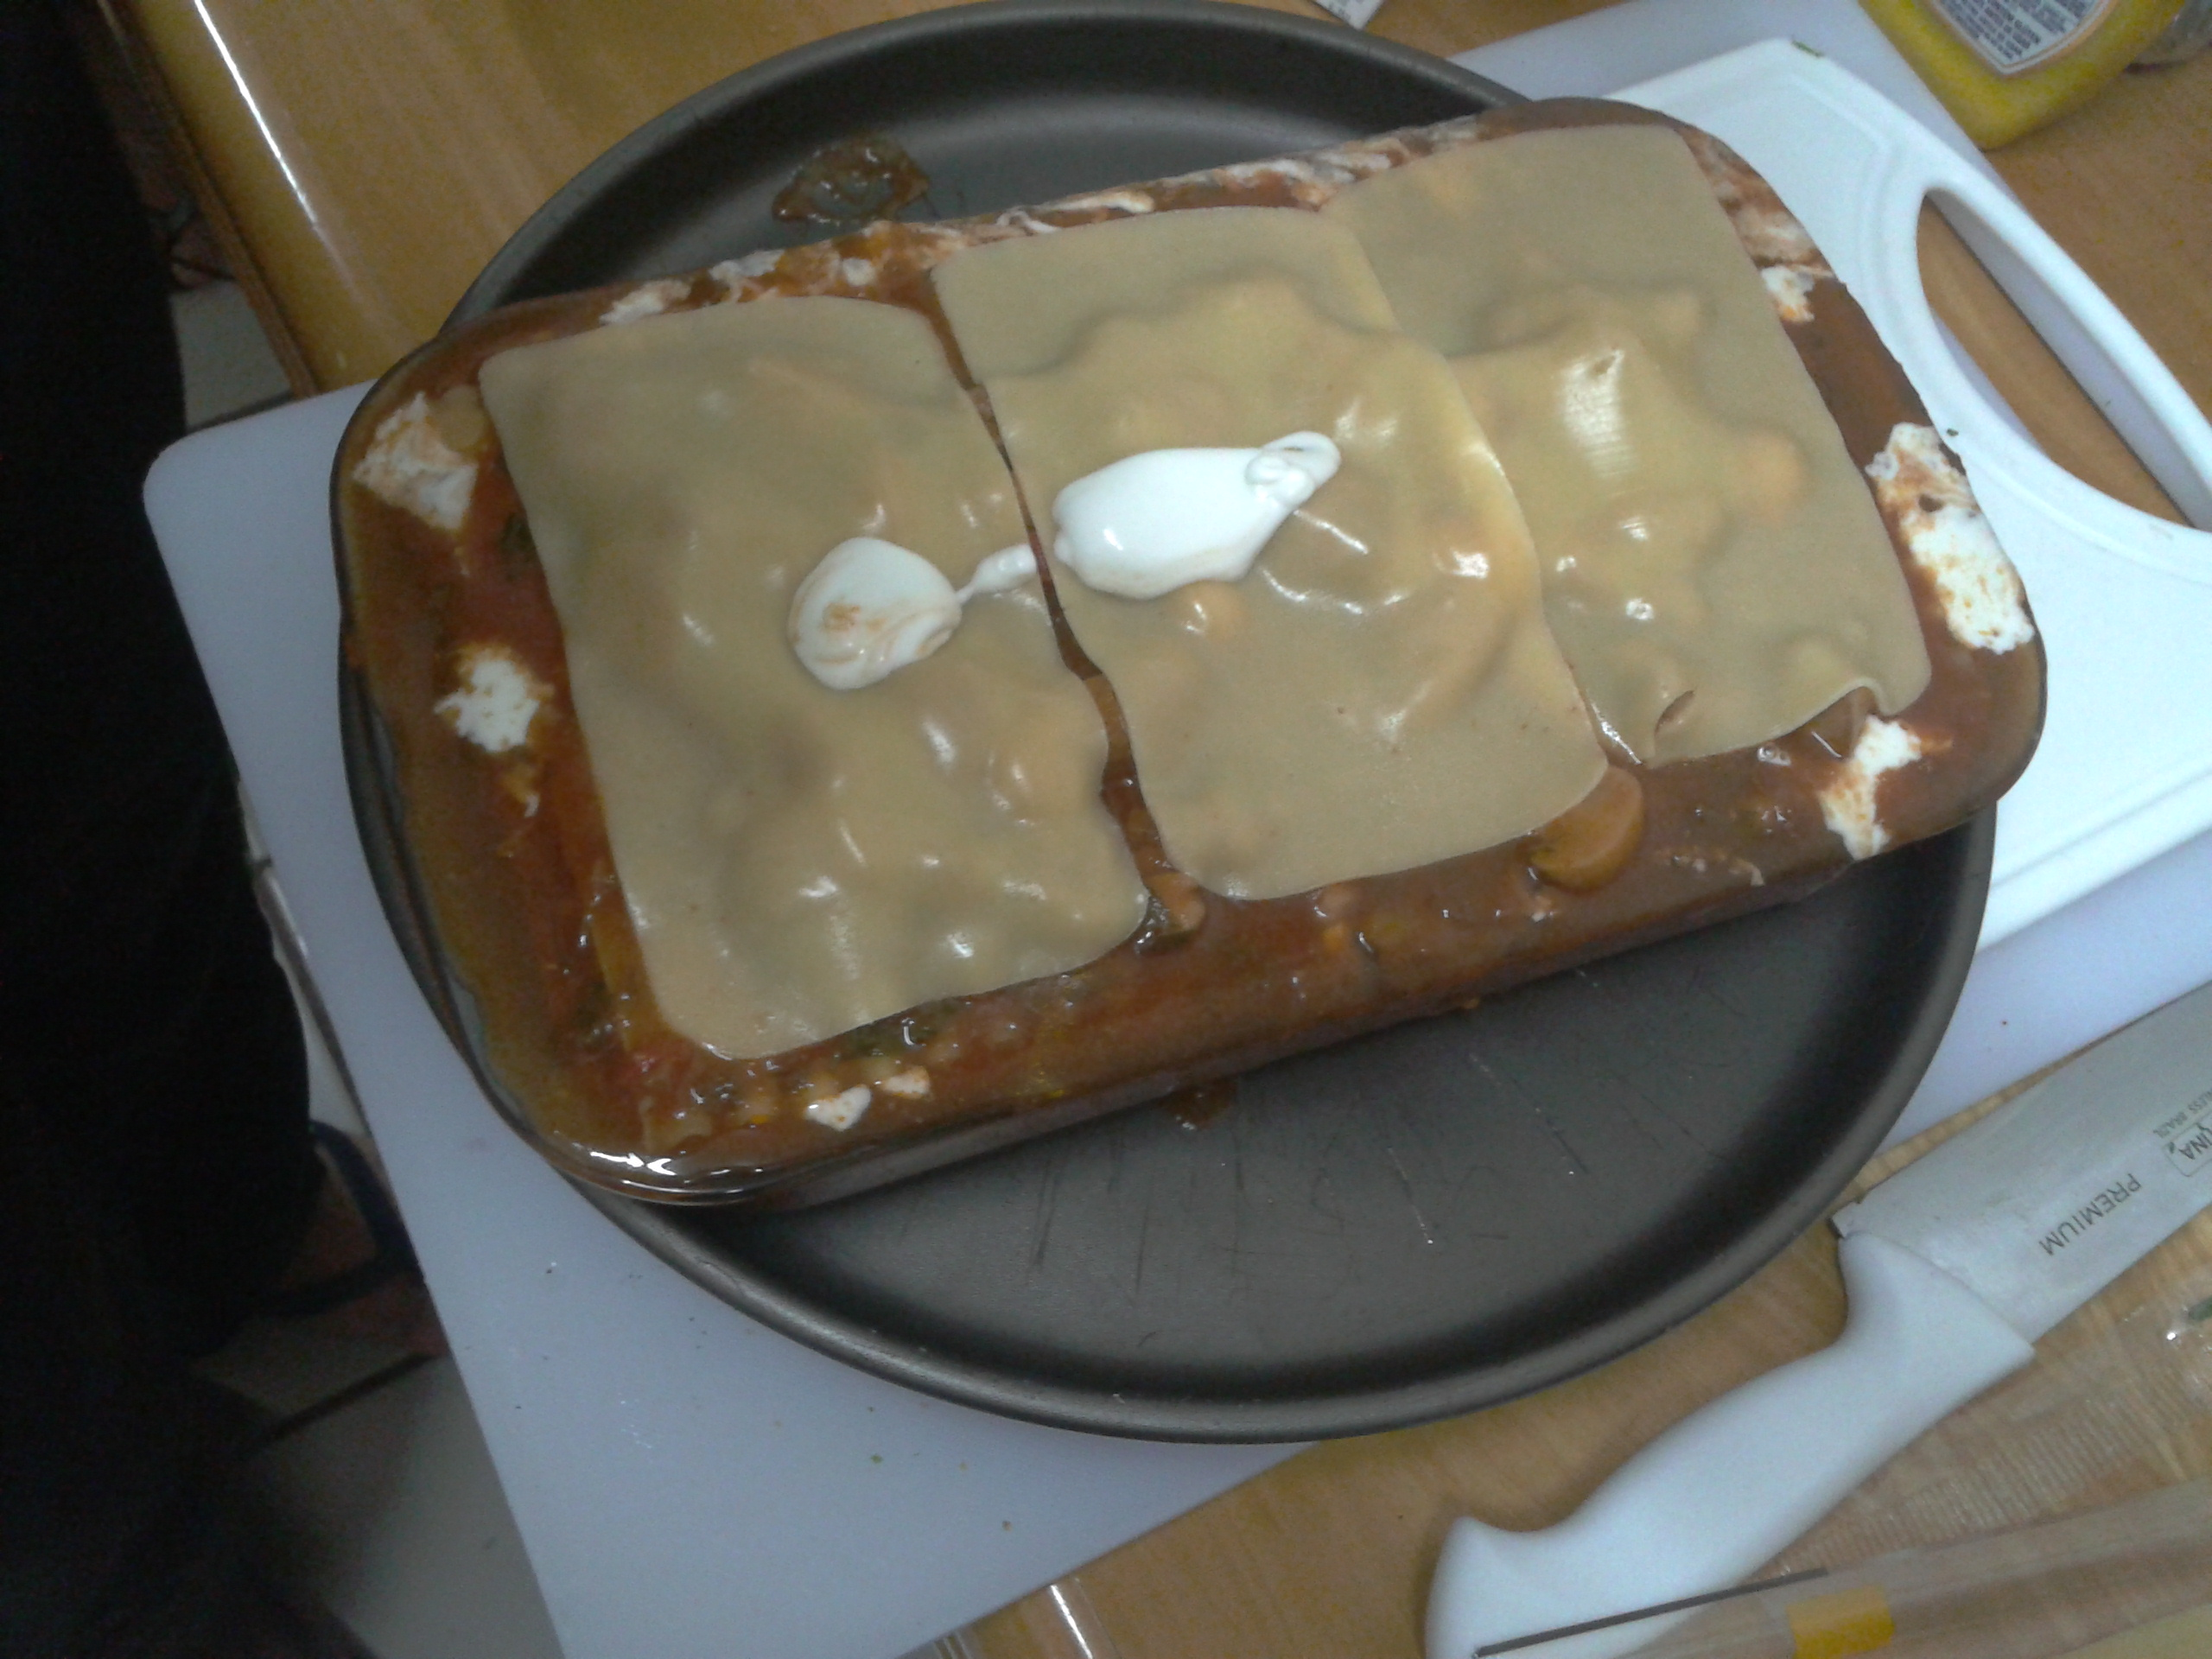
\includegraphics[width = \textwidth]{./figuraA.jpg}
	\caption{fome...}
	\label{fig:lasanha}
\end{figure}
A figura da lasanha é a figura \ref{fig:lasanha}

\chapter{Capítulo Aleatório}
\label{chap:CapAle}

Lista do capítulo da lista \ref{chap:CapAle}:

\begin{enumerate}
\item item a
\item item b
\item item c
	\begin{itemize}
	\item item d
	\item item e
	\item item f
		\begin{enumerate}[label*=\arabic*.]
		\item item g
		\item item h
		\item item i
			\begin{itemize}
			\item itemizeception
			\end{itemize}
		\end{enumerate}
	\end{itemize}
\end{enumerate}

CIRCUITÃO:

\begin{figure}[!htb] \label{fig:circuitevers}
\centering
\begin{tikzpicture}

\draw (0,0) to [sV] (0,2) to[closing switch] (2,2) to[lamp] (2,0) -- (0,0);
\draw (3,0)  to[R] (3,3);

\end{tikzpicture}
\caption{circuto massa}
\end{figure}

Juntando sem pular linha: 70~cm 
\hfill

\begin{tikzpicture}
\centering
\begin{axis}[xlabel=eixo x,ylabel=eixo y]
\addplot+[domain=0:0.5]{x*x -18};
\end{axis}
\end{tikzpicture}



\end{document}